% !TEX root = ../tex/2-2.tex
\section{2.2 変分的観点：DDPM}

\begin{frame}{2.2 変分的観点：DDPM}
    \begin{block}{Denoising Diffusion Probabilistic Model}
        DDPMは、データをノイズへ変える過程と、
        ノイズをデータへ戻す過程を組み合わせた生成モデルである。
    \end{block}
    \begin{itemize}
        \item VAE・HVAEと同様に、変分的な枠組みに基づく
        \item 符号化に相当する順方向過程は固定する
        \item 生成に相当する逆方向過程だけを学習する
        \item 一度に生成せず、小さなノイズ除去を繰り返す
    \end{itemize}
    \vfill
    \footnotesize
    Sohl-Dickstein et al.\ (2015), Ho et al.\ (2020)
\end{frame}
%=============================================
\begin{frame}{DDPMを構成する二つの確率過程}
    \begin{columns}[T,onlytextwidth]
        \begin{column}{0.48\textwidth}
            \begin{block}{順方向過程}
                \centering
                \textbf{固定されたエンコーダ}
                \[
                    p(\boldsymbol{x}_i\mid\boldsymbol{x}_{i-1})
                \]
                \begin{itemize}
                    \item データへガウスノイズを加える
                    \item 徐々に情報を失わせる
                    \item パラメータは学習しない
                \end{itemize}
            \end{block}
        \end{column}
        \begin{column}{0.48\textwidth}
            \begin{exampleblock}{逆方向過程}
                \centering
                \textbf{学習可能なデコーダ}
                \[
                    p_\phi(\boldsymbol{x}_{i-1}\mid\boldsymbol{x}_i)
                \]
                \begin{itemize}
                    \item ノイズを段階的に除去する
                    \item 純粋なノイズから生成する
                    \item ニューラルネットワークで学習
                \end{itemize}
            \end{exampleblock}
        \end{column}
    \end{columns}
\end{frame}
%=============================================
\begin{frame}{図2.3：DDPMの概略図}
    \centering
    \begin{tikzpicture}[
        state/.style={circle,draw=main,very thick,minimum size=10mm},
        fwd/.style={->,very thick,gray!75},
        rev/.style={->,very thick,examplecol},
        every node/.style={font=\small}
    ]
        \node[state] (x0) at (0,0) {$\boldsymbol{x}_0$};
        \node[state] (x1) at (2.4,0) {$\boldsymbol{x}_1$};
        \node[state] (x2) at (4.8,0) {$\boldsymbol{x}_2$};
        \node (dots) at (6.6,0) {$\cdots$};
        \node[state] (xl) at (8.4,0) {$\boldsymbol{x}_L$};

        \draw[fwd] ([yshift=1.5mm]x0.east) --
            node[above] {$p(\boldsymbol{x}_1\mid\boldsymbol{x}_0)$}
            ([yshift=1.5mm]x1.west);
        \draw[fwd] ([yshift=1.5mm]x1.east) --
            node[above] {$p(\boldsymbol{x}_2\mid\boldsymbol{x}_1)$}
            ([yshift=1.5mm]x2.west);
        \draw[fwd] ([yshift=1.5mm]x2.east) -- ([yshift=1.5mm]dots.west);
        \draw[fwd] ([yshift=1.5mm]dots.east) -- ([yshift=1.5mm]xl.west);

        \draw[rev] ([yshift=-1.5mm]x1.west) --
            node[below] {$p_\phi(\boldsymbol{x}_0\mid\boldsymbol{x}_1)$}
            ([yshift=-1.5mm]x0.east);
        \draw[rev] ([yshift=-1.5mm]x2.west) --
            node[below] {$p_\phi(\boldsymbol{x}_1\mid\boldsymbol{x}_2)$}
            ([yshift=-1.5mm]x1.east);
        \draw[rev] ([yshift=-1.5mm]dots.west) -- ([yshift=-1.5mm]x2.east);
        \draw[rev] ([yshift=-1.5mm]xl.west) -- ([yshift=-1.5mm]dots.east);

        \node[gray!75] at (4.2,1.25) {順方向：固定されたノイズ付加};
        \node[examplecol] at (4.2,-1.25) {逆方向：学習するノイズ除去};
    \end{tikzpicture}
    \vfill
    \begin{itemize}
        \item $\boldsymbol{x}_0$は実データ、$\boldsymbol{x}_L$はほぼ純粋なノイズ
        \item 逆方向では、各ステップの小さな変化だけを学習すればよい
    \end{itemize}
\end{frame}
%=============================================
\begin{frame}{なぜ段階的な生成にするのか}
    \begin{columns}[c,onlytextwidth]
        \begin{column}{0.46\textwidth}
            \begin{alertblock}{一度に生成}
                \[
                    \boldsymbol{z}\longrightarrow\boldsymbol{x}
                \]
                ノイズや潜在表現から、複雑なデータ全体を
                一度に構成する必要がある。
            \end{alertblock}
        \end{column}
        \begin{column}{0.08\textwidth}
            \centering
            \Large $\Longrightarrow$
        \end{column}
        \begin{column}{0.46\textwidth}
            \begin{exampleblock}{段階的に生成}
                \[
                    \boldsymbol{x}_i\longrightarrow\boldsymbol{x}_{i-1}
                \]
                各ステップでは、少量のノイズによる変化だけを
                逆転させればよい。
            \end{exampleblock}
        \end{column}
    \end{columns}
    \vfill
    \begin{block}{DDPMの工夫}
        エンコーダを固定し、扱いやすい局所的なノイズ除去へ
        学習能力を集中させる。
    \end{block}
\end{frame}
%=============================================
\begin{frame}{図2.4：順方向過程によるノイズの増加}
    \centering
    \begin{columns}[c,onlytextwidth]
        \begin{column}{0.172\textwidth}
            \centering
            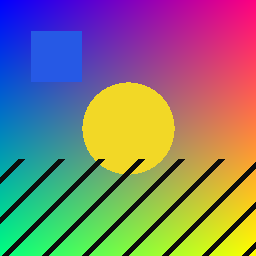
\includegraphics[width=\linewidth]
            {../../ch01-dgm/experiments/noise-level/vary-t-vp/outputs/vp_t0p0.png}\\
            $\boldsymbol{x}_0$\\[-1mm]
            \scriptsize 元データ
        \end{column}
        \begin{column}{0.035\textwidth}\centering$\rightarrow$\end{column}
        \begin{column}{0.172\textwidth}
            \centering
            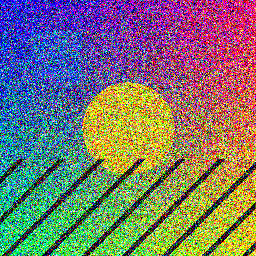
\includegraphics[width=\linewidth]
            {../../ch01-dgm/experiments/noise-level/vary-t-vp/outputs/vp_t0p4.png}\\
            $\boldsymbol{x}_1$\\[-1mm]
            \scriptsize 少量のノイズ
        \end{column}
        \begin{column}{0.035\textwidth}\centering$\rightarrow$\end{column}
        \begin{column}{0.172\textwidth}
            \centering
            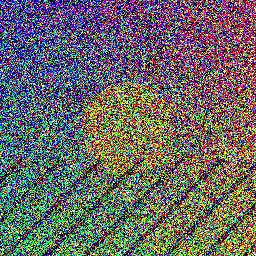
\includegraphics[width=\linewidth]
            {../../ch01-dgm/experiments/noise-level/vary-t-vp/outputs/vp_t0p8.png}\\
            $\boldsymbol{x}_2$\\[-1mm]
            \scriptsize ノイズ増加
        \end{column}
        \begin{column}{0.035\textwidth}\centering$\rightarrow$\end{column}
        \begin{column}{0.172\textwidth}
            \centering
            
\includegraphics[width=\linewidth]
            {../../ch01-dgm/experiments/noise-level/vary-t-vp/outputs/vp_t0p95.png}\\
            $\boldsymbol{x}_{L-1}$\\[-1mm]
            \scriptsize ほぼノイズ
        \end{column}
        \begin{column}{0.035\textwidth}\centering$\rightarrow$\end{column}
        \begin{column}{0.172\textwidth}
            \centering
            
\includegraphics[width=\linewidth]
            {../../ch01-dgm/experiments/noise-level/vary-t-vp/outputs/vp_t1p0.png}\\
            $\boldsymbol{x}_L$\\[-1mm]
            \scriptsize 純粋なノイズ
        \end{column}
    \end{columns}
    \vfill
    ガウスノイズを段階的に加え、
    データ分布を単純なノイズ分布へ近づける。
\end{frame}
%=============================================
\subsection{2.2.1 固定された順方向過程}
\begin{frame}{固定されたガウス遷移}
    順方向過程の各ステップを、次の遷移カーネルで定める。
    \[
        \boxed{
        p(\boldsymbol{x}_i\mid\boldsymbol{x}_{i-1})
        :=
        \mathcal{N}\!\left(
        \boldsymbol{x}_i;\,
        \sqrt{1-\beta_i^2}\,\boldsymbol{x}_{i-1},
        \beta_i^2\boldsymbol{I}
        \right)
        }
    \]
    \[
        \alpha_i:=\sqrt{1-\beta_i^2}
    \]
    と定義すれば、
    \[
        \boldsymbol{x}_i\mid\boldsymbol{x}_{i-1}
        \sim
        \mathcal{N}\!\left(
        \alpha_i\boldsymbol{x}_{i-1},
        \beta_i^2\boldsymbol{I}
        \right).
    \]
    \begin{itemize}
        \item $\{\beta_i\}_{i=1}^{L}$：あらかじめ定めるノイズスケジュール
        \item $\beta_i\in(0,1)$：ステップ$i$で加えるノイズの大きさ
        \item この順方向遷移には学習パラメータがない
    \end{itemize}
\end{frame}
%=============================================
\begin{frame}{分布の定義と更新式は等価}
    標準ガウスノイズを用意する。
    \[
        \boldsymbol{\epsilon}_i\sim\mathcal{N}(\boldsymbol{0},\boldsymbol{I})
    \]
    すると、遷移カーネルからのサンプリングは
    \[
        \boxed{
        \boldsymbol{x}_i
        =
        \alpha_i\boldsymbol{x}_{i-1}
        +
        \beta_i\boldsymbol{\epsilon}_i
        }
    \]
    と書ける。
    \begin{align*}
        \mathbb{E}[\boldsymbol{x}_i\mid\boldsymbol{x}_{i-1}]
        &=\alpha_i\boldsymbol{x}_{i-1},\\
        \operatorname{Cov}(\boldsymbol{x}_i\mid\boldsymbol{x}_{i-1})
        &=\beta_i^2\boldsymbol{I}.
    \end{align*}
    \begin{exampleblock}{直感}
        前の状態を$\alpha_i$倍して少し弱め、
        独立なノイズを$\beta_i$倍して加える。
    \end{exampleblock}
\end{frame}
%=============================================
\begin{frame}{係数の関係と分散の保存}
    定義より、
    \[
        \boxed{\alpha_i^2+\beta_i^2=1}
    \]
    が成り立つ。
    \begin{block}{標準ガウス分布はこの更新で保存される}
        $\boldsymbol{x}_{i-1}\sim\mathcal{N}(\boldsymbol{0},\boldsymbol{I})$、
        $\boldsymbol{\epsilon}_i\sim\mathcal{N}(\boldsymbol{0},\boldsymbol{I})$
        が独立なら、
        \[
            \operatorname{Cov}(\boldsymbol{x}_i)
            =
            \alpha_i^2\boldsymbol{I}
            +
            \beta_i^2\boldsymbol{I}
            =
            \boldsymbol{I}.
        \]
    \end{block}
    \begin{alertblock}{記法上の注意}
        ここではノイズ分散を$\beta_i^2$と書いている。
        文献によっては分散そのものを$\beta_i$と表すため、
        $\sqrt{1-\beta_i}$という式が現れる。
    \end{alertblock}
\end{frame}
%=============================================
\begin{frame}{摂動カーネル：任意の時点へ直接進む}
    遷移を繰り返したときの累積信号係数を
    \[
        \bar{\alpha}_i
        :=
        \prod_{k=1}^{i}\alpha_k
        =
        \prod_{k=1}^{i}\sqrt{1-\beta_k^2}
    \]
    と定義する。すると、
    \[
        \boxed{
        p_i(\boldsymbol{x}_i\mid\boldsymbol{x}_0)
        =
        \mathcal{N}\!\left(
        \boldsymbol{x}_i;\,
        \bar{\alpha}_i\boldsymbol{x}_0,\,
        (1-\bar{\alpha}_i^2)\boldsymbol{I}
        \right)
        }
    \]
    を得る。
    \begin{block}{重要}
        $\boldsymbol{x}_1,\ldots,\boldsymbol{x}_{i-1}$を計算せず、
        $\boldsymbol{x}_0$から任意の$\boldsymbol{x}_i$を直接生成できる。
    \end{block}
\end{frame}
%=============================================
\begin{frame}{直接サンプリングする式}
    摂動カーネルは、次の更新式と等価である。
    \[
        \boxed{
        \boldsymbol{x}_i
        =
        \bar{\alpha}_i\boldsymbol{x}_0
        +
        \sqrt{1-\bar{\alpha}_i^2}\,
        \boldsymbol{\epsilon},
        \qquad
        \boldsymbol{\epsilon}
        \sim\mathcal{N}(\boldsymbol{0},\boldsymbol{I})
        }
        \tag{2.2.1}
    \]
    \begin{columns}[T,onlytextwidth]
        \begin{column}{0.47\textwidth}
            \begin{alertblock}{逐次計算}
                \[
                    \boldsymbol{x}_0\to\boldsymbol{x}_1
                    \to\cdots\to\boldsymbol{x}_i
                \]
                前の状態が毎回必要。
            \end{alertblock}
        \end{column}
        \begin{column}{0.47\textwidth}
            \begin{exampleblock}{直接計算}
                \[
                    \boldsymbol{x}_0\longrightarrow\boldsymbol{x}_i
                \]
                学習時に効率よくノイズを加えられる。
            \end{exampleblock}
        \end{column}
    \end{columns}
\end{frame}
%=============================================
\begin{frame}{なぜ複数のノイズを一つにまとめられるのか}
    例として2ステップ展開する。
    \begin{align*}
        \boldsymbol{x}_2
        &=
        \alpha_2\boldsymbol{x}_1+\beta_2\boldsymbol{\epsilon}_2\\
        &=
        \alpha_2\alpha_1\boldsymbol{x}_0
        +
        \alpha_2\beta_1\boldsymbol{\epsilon}_1
        +
        \beta_2\boldsymbol{\epsilon}_2.
    \end{align*}
    独立なガウス変数の線形結合もガウス分布に従う。
    ノイズ部分の共分散は、
    \[
        (\alpha_2^2\beta_1^2+\beta_2^2)\boldsymbol{I}
        =
        (1-\alpha_1^2\alpha_2^2)\boldsymbol{I}.
    \]
    したがって、
    \[
        \boldsymbol{x}_2
        \overset{d}{=}
        \bar{\alpha}_2\boldsymbol{x}_0
        +
        \sqrt{1-\bar{\alpha}_2^2}\,\boldsymbol{\epsilon}.
    \]
    \footnotesize
    $\overset{d}{=}$は「同じ分布に従う」ことを表す。
\end{frame}
%=============================================
\begin{frame}{順方向過程の終点と事前分布}
    式（2.2.1）を信号成分とノイズ成分に分ける。
    \[
        \boldsymbol{x}_i
        =
        \underbrace{\bar{\alpha}_i\boldsymbol{x}_0}_{\text{元データの成分}}
        +
        \underbrace{
        \sqrt{1-\bar{\alpha}_i^2}\boldsymbol{\epsilon}
        }_{\text{ノイズ成分}}
    \]
    適切なスケジュールによって$\bar{\alpha}_L\approx0$とすれば、
    \[
        \boldsymbol{x}_L\approx\boldsymbol{\epsilon}
        \sim\mathcal{N}(\boldsymbol{0},\boldsymbol{I}).
    \]
    したがって、生成の出発点として
    \[
        \boxed{
        p_{\mathrm{prior}}
        :=
        \mathcal{N}(\boldsymbol{0},\boldsymbol{I})
        }
    \]
    を選べる。
    \begin{alertblock}{注意}
        $\beta_i$が単調増加するだけでは不十分であり、
        $\bar{\alpha}_L$が十分小さくなるスケジュールが必要である。
    \end{alertblock}
\end{frame}
%=============================================
\subsection{2.2.2 学習可能な逆方向過程}
\begin{frame}{逆方向ノイズ除去過程}
    生成時には、純粋なノイズから出発する。
    \[
        \boldsymbol{x}_L\sim p_{\mathrm{prior}}
    \]
    そして、$i=L,\ldots,1$について、
    \[
        \boldsymbol{x}_{i-1}
        \sim
        p_\phi(\boldsymbol{x}_{i-1}\mid\boldsymbol{x}_i)
    \]
    と段階的にサンプリングする。
    \begin{block}{学習の目標}
        モデルの逆方向遷移
        $p_\phi(\boldsymbol{x}_{i-1}\mid\boldsymbol{x}_i)$を、
        真の逆方向遷移
        $p(\boldsymbol{x}_{i-1}\mid\boldsymbol{x}_i)$へ近づける。
    \end{block}
    \[
        p_\phi(\boldsymbol{x}_{i-1}\mid\boldsymbol{x}_i)
        \approx
        p(\boldsymbol{x}_{i-1}\mid\boldsymbol{x}_i)
    \]
\end{frame}
%=============================================
\begin{frame}{図2.5：逆方向過程の概略図}
    \centering
    \begin{tikzpicture}[
        state/.style={circle,draw=main,very thick,minimum size=11mm},
        arr/.style={->,very thick,examplecol},
        every node/.style={font=\small}
    ]
        \node[state,fill=gray!35] (xl) at (0,0) {$\boldsymbol{x}_L$};
        \node[state,fill=gray!25] (xa) at (2.1,0) {$\boldsymbol{x}_{L-1}$};
        \node (dots) at (4.0,0) {$\cdots$};
        \node[state,fill=main!12] (x1) at (5.9,0) {$\boldsymbol{x}_1$};
        \node[state,fill=main!25] (x0) at (8.0,0) {$\boldsymbol{x}_0$};

        \draw[arr] (xl) -- node[above] {$p_\phi$} (xa);
        \draw[arr] (xa) -- (dots);
        \draw[arr] (dots) -- (x1);
        \draw[arr] (x1) -- node[above] {$p_\phi$} (x0);

        \node at (0,-1.0) {ノイズ};
        \node at (2.1,-1.0) {粗い構造};
        \node at (5.9,-1.0) {細部};
        \node at (8.0,-1.0) {生成データ};
    \end{tikzpicture}
    \vfill
    各ステップで現在の状態だけを使うため、逆方向過程も
    マルコフ連鎖としてモデル化される。
\end{frame}
%=============================================
\begin{frame}{なぜ真の逆方向遷移は未知なのか}
    ベイズの定理より、形式的には
    \[
        p(\boldsymbol{x}_{i-1}\mid\boldsymbol{x}_i)
        =
        \frac{
        p(\boldsymbol{x}_i\mid\boldsymbol{x}_{i-1})
        p_{i-1}(\boldsymbol{x}_{i-1})
        }{
        p_i(\boldsymbol{x}_i)
        }
    \]
    と書ける。
    \begin{itemize}
        \item $p(\boldsymbol{x}_i\mid\boldsymbol{x}_{i-1})$：
        固定したので既知
        \item $p_{i-1}(\boldsymbol{x}_{i-1})$：
        実データに依存する周辺分布
        \item $p_i(\boldsymbol{x}_i)$：
        実データに依存する周辺分布
    \end{itemize}
    \[
        p_i(\boldsymbol{x}_i)
        =
        \int
        p_i(\boldsymbol{x}_i\mid\boldsymbol{x}_0)
        p_{\mathrm{data}}(\boldsymbol{x}_0)
        \,d\boldsymbol{x}_0
    \]
    \begin{alertblock}{問題}
        $p_{\mathrm{data}}$の密度は未知なので、
        これらの周辺分布を閉形式で評価できない。
    \end{alertblock}
\end{frame}
%=============================================
\begin{frame}{直接考えた学習目的}
    未知の真の逆方向遷移をモデルで近似するため、
    次の期待KLダイバージェンスを考える。
    \[
        \boxed{
        \mathbb{E}_{p_i(\boldsymbol{x}_i)}
        \left[
        D_{\mathrm{KL}}\!\left(
        p(\boldsymbol{x}_{i-1}\mid\boldsymbol{x}_i)
        \,\|\,
        p_\phi(\boldsymbol{x}_{i-1}\mid\boldsymbol{x}_i)
        \right)
        \right]
        }
        \tag{2.2.2}
    \]
    \begin{exampleblock}{目的}
        観測された$\boldsymbol{x}_i$から、
        一段階前の$\boldsymbol{x}_{i-1}$の分布を予測する。
    \end{exampleblock}
    \begin{alertblock}{そのままでは計算できない}
        KLの第1引数
        $p(\boldsymbol{x}_{i-1}\mid\boldsymbol{x}_i)$自体が、
        未知の周辺分布を含む。
    \end{alertblock}
\end{frame}
%=============================================
\begin{frame}{条件付けの工夫}
    学習時には、ノイズ付加の出発点
    $\boldsymbol{x}_0$を知っている。
    \begin{columns}[T,onlytextwidth]
        \begin{column}{0.47\textwidth}
            \begin{alertblock}{計算困難}
                \[
                    p(\boldsymbol{x}_{i-1}\mid\boldsymbol{x}_i)
                \]
                あらゆる元データの可能性を平均した、
                複雑な混合分布になり得る。
            \end{alertblock}
        \end{column}
        \begin{column}{0.47\textwidth}
            \begin{exampleblock}{計算可能}
                \[
                    p(\boldsymbol{x}_{i-1}
                    \mid\boldsymbol{x}_i,\boldsymbol{x}_0)
                \]
                元データを固定すると、
                平均と分散を解析的に求められるガウス分布になる。
            \end{exampleblock}
        \end{column}
    \end{columns}
    \vfill
    \[
        \text{未知の周辺逆遷移}
        \quad\Longrightarrow\quad
        \text{既知のデータで条件付けた逆遷移}
    \]
\end{frame}
%=============================================
\begin{frame}{図2.6：条件付けによって単純になる}
    \centering
    \begin{tikzpicture}[
        every node/.style={font=\small},
        axis/.style={->,gray!70},
        mix/.style={draw=alertcol,thick,fill=alertcol!10},
        single/.style={draw=examplecol,very thick,fill=examplecol!12}
    ]
        \begin{scope}[xshift=0cm]
            \draw[axis] (-0.2,0) -- (4.2,0);
            \draw[axis] (0,-0.2) -- (0,2.5);
            \draw[mix] (0.5,0) .. controls (0.9,0.1) and (0.9,1.8) ..
                (1.35,0) -- cycle;
            \draw[mix] (1.6,0) .. controls (2.1,0.15) and (2.15,2.25) ..
                (2.7,0) -- cycle;
            \draw[mix] (2.7,0) .. controls (3.15,0.1) and (3.35,1.5) ..
                (3.8,0) -- cycle;
            \node[align=center] at (2,-0.65)
                {$p(\boldsymbol{x}_{i-1}\mid\boldsymbol{x}_i)$\\
                複数候補の混合};
        \end{scope}

        \draw[->,very thick] (4.55,1.2) -- node[above] {$+\boldsymbol{x}_0$} (5.65,1.2);

        \begin{scope}[xshift=6cm]
            \draw[axis] (-0.2,0) -- (4.2,0);
            \draw[axis] (0,-0.2) -- (0,2.5);
            \draw[single] (1.0,0) .. controls (1.65,0.15) and (2.05,2.3) ..
                (3.1,0) -- cycle;
            \node[align=center] at (2,-0.65)
                {$p(\boldsymbol{x}_{i-1}\mid\boldsymbol{x}_i,\boldsymbol{x}_0)$\\
                単一のガウス分布};
        \end{scope}
    \end{tikzpicture}
    \vfill
    元データを条件へ加えることで、
    複雑な周辺分布を扱いやすい学習目標へ変換する。
\end{frame}
%=============================================
\begin{frame}{なぜ条件付き分布は計算できるのか}
    順方向過程では、次の二つが既知のガウス分布である。
    \[
        p(\boldsymbol{x}_i\mid\boldsymbol{x}_{i-1})
        \quad\text{と}\quad
        p_{i-1}(\boldsymbol{x}_{i-1}\mid\boldsymbol{x}_0)
    \]
    ベイズの定理から、
    \[
        p(\boldsymbol{x}_{i-1}\mid
        \boldsymbol{x}_i,\boldsymbol{x}_0)
        \propto
        p(\boldsymbol{x}_i\mid\boldsymbol{x}_{i-1})
        p_{i-1}(\boldsymbol{x}_{i-1}\mid\boldsymbol{x}_0).
    \]
    ガウス密度どうしの積は、正規化すると再びガウス分布になる。
    \[
        p(\boldsymbol{x}_{i-1}\mid
        \boldsymbol{x}_i,\boldsymbol{x}_0)
        =
        \mathcal{N}\!\left(
        \boldsymbol{x}_{i-1};
        \text{計算可能な平均},
        \text{計算可能な共分散}
        \right)
    \]
    \begin{block}{結果}
        学習用に生成した
        $(\boldsymbol{x}_0,\boldsymbol{x}_i)$から、
        一段階前の分布を解析的な教師として作れる。
    \end{block}
\end{frame}
%=============================================
\begin{frame}{条件付き分布と周辺分布の関係}
    一つの$\boldsymbol{x}_0$へ条件付けた分布は、
    本来の周辺逆遷移と同じではない。
    \[
        \boxed{
        p(\boldsymbol{x}_{i-1}\mid\boldsymbol{x}_i)
        =
        \int
        p(\boldsymbol{x}_{i-1}\mid
        \boldsymbol{x}_i,\boldsymbol{x}_0)
        p(\boldsymbol{x}_0\mid\boldsymbol{x}_i)
        \,d\boldsymbol{x}_0
        }
    \]
    \begin{itemize}
        \item 各$\boldsymbol{x}_0$に条件付けた分布：
        単純なガウス分布
        \item それらを$p(\boldsymbol{x}_0\mid\boldsymbol{x}_i)$で平均：
        本来求めたい周辺逆遷移
        \item 多数の訓練例で条件付き目的を平均すると、
        周辺目的と同じ最適予測を学習できる
    \end{itemize}
\end{frame}
%=============================================
\begin{frame}{2.2前半のまとめ}
    \begin{enumerate}
        \item 順方向過程は、固定ガウス遷移でデータへノイズを加える
        \[
            \boldsymbol{x}_i
            =\alpha_i\boldsymbol{x}_{i-1}
            +\beta_i\boldsymbol{\epsilon}_i
        \]
        \item 任意の時点へ直接サンプリングできる
        \[
            \boldsymbol{x}_i
            =\bar{\alpha}_i\boldsymbol{x}_0
            +\sqrt{1-\bar{\alpha}_i^2}\boldsymbol{\epsilon}
        \]
        \item 真の逆方向遷移は、未知の周辺分布を含むため計算困難
        \item 学習時に既知の$\boldsymbol{x}_0$で条件付けると、
        計算可能なガウス分布になる
    \end{enumerate}
    \begin{exampleblock}{中心となる考え方}
        未知の分布を直接求める問題を、
        既知の元データで条件付けた回帰問題へ変換する。
    \end{exampleblock}
\end{frame}
